% !TEX options=--shell-escape
\documentclass [12pt]{article} 
\usepackage {amsmath}
\usepackage {amsthm}
\usepackage {amssymb}
\usepackage {graphicx} 
\usepackage {float}
\usepackage {multirow}
\usepackage {xcolor}
\usepackage {algorithmic}
\usepackage [ruled,vlined,commentsnumbered,titlenotnumbered]{algorithm2e} \usepackage {array} 
\usepackage {booktabs} 
\usepackage {url} 
\usepackage {parskip} 
\usepackage [margin=1in]{geometry} 
\usepackage [T1]{fontenc} 
\usepackage {cmbright} 
\usepackage [many]{tcolorbox} 
\usepackage [colorlinks = true,
            linkcolor = blue,
            urlcolor  = blue,
            citecolor = blue,
            anchorcolor = blue]{hyperref} 
\usepackage {enumitem} 
\usepackage {xparse} 
\usepackage {verbatim}
\usepackage{listings}
\usepackage{xcolor}
\usepackage{csquotes}
\usepackage[cache=false]{minted}
\usepackage{mdframed}
\usepackage{tikz}
\usetikzlibrary{shapes.symbols}
\newtheorem{theorem}{Theorem}

\DeclareTColorBox {Solution}{}{breakable, title={Solution}}
\DeclareTColorBox {Solution*}{}{breakable, title={Solution (provided)}}
\DeclareTColorBox {Instruction}{}{boxrule=0pt, boxsep=0pt, left=0.5em, right=0.5em, top=0.5em, bottom=0.5em, arc=0pt, toprule=1pt, bottomrule=1pt}
\DeclareDocumentCommand {\Expecting }{+m}{\textbf {[We are expecting:} #1\textbf {]}}
\DeclareDocumentCommand {\Points }{m}{\textbf {(#1 pt.)}} 
\newcommand {\hint }[1]{\noindent {[\textbf {HINT:} \em #1 \em ]}} \newcommand {\pts }[1]{\textbf {(#1 pt.)}} 

\begin{document} 

{\LARGE \textbf {COMP 285 (NC A\&T, Spr `22)}\hfill \textbf {Weekly Quiz 9} } 

\begin{Instruction}

\paragraph{Reporting Issues} If you find any issues with the solutions, reach out to Chi Wang (author) or Luis Perez (reviewer).

\end{Instruction}


\section{} We are computing the longest common subsequence between two strings of length four $S = X_1X_2X_3X_4$ and $T = Y_1Y_2Y_3Y_4$. We fill the array $C$ where $C_{i ,j}$ is the length of the longest common subsequence between the prefix of length $i$ from $S$ and the prefix of length $j$ from $T$. The array $C$ can be found below with some entries masked. What can be said about $X_1$ and $Y_4$ (the first character of S and the last character of Y)?


\begin{figure}[H]
    \centering
    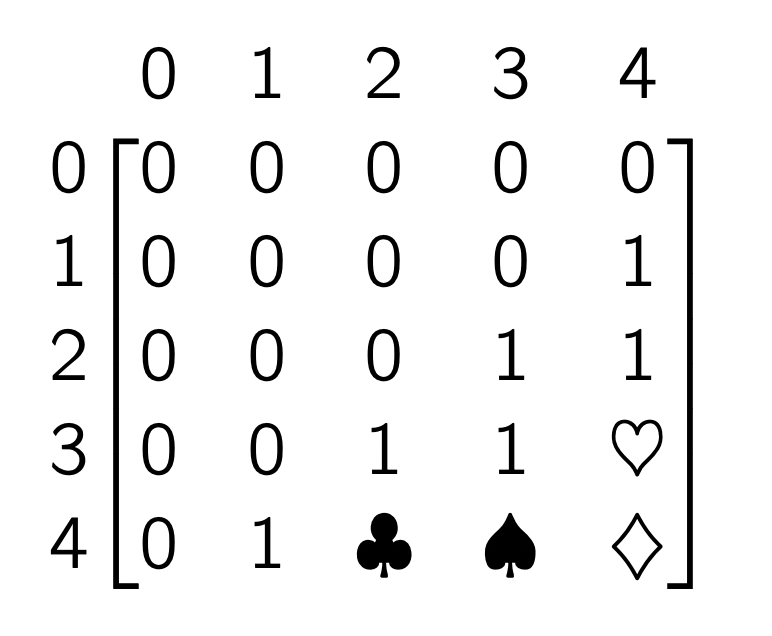
\includegraphics[scale=0.5]{9.png} 
    \label{fig:my_label}
\end{figure}

\begin{Solution}
The characters are equal. We can see this by looking at row $1$. It is all $0$'s until we get to column 4, which means that $X_1$ matched none of the characters in $Y$ except for $Y_4$.
\end{Solution}


\section{} What can be said about $X_2 $ and $Y_3$?

\begin{Solution}
By a similar argument, if we look at row labeled 2, it is all 0s until we reach the column labeled 3. As such, this is where it matched with $Y_3$. So the two characters are equal.
\end{Solution}


\section{} What can be said about $X_2$ and $Y_4$?

\begin{Solution}
Suppose $X_2$ matches $Y_4$. By row $2$, we know that $X_2$ matches $Y_3$. However, that would mean $Y_3$ and $Y_4$ are the same character, but if we look at row $1$, we see that $X_1$ only matches $Y_4$, which means $Y_4 \neq Y_3$, as asuch $X_2 \neq Y_4$.
\end{Solution}


\section{} What is the value of the heart?

\begin{Solution}
We're basically asking whether $X_3$ matches $Y_4$. We know that $Y_4$ does not match any other characters in $Y$. However, we see that $X_3$ matches $Y_2$. As such, $X_3$ cannot match $Y_4$.

This means the hearth has a value of $1$ (max of the up and left cells).
\end{Solution}


\section{} What is the value of the spade?
\begin{Solution}
We're asking if $X_4$ matches $Y_3$. We know already that $Y_3$ does not match any other characters in $Y$ (this is clear from row labeled 2). However, $X_4$ matches $Y_1$. As such, $X_4$ does not match $Y_3$.

Therefore, the spade has a value of $1$ (max of the up and left cells).
\end{Solution}


\section{} What is the value of the clubs?

\begin{Solution}
This is asking if $X_4$ matches $Y_2$. We know $Y_2$ matches $X_3$ and $X_4$ matches $Y_1$. However, we know $X_3$ does not match $Y_1$. Therfore $X_4$ doe snot match $Y_2$.

Therefore, the clubs has a value of $1$ (max of the up and left cells).
\end{Solution}


\section{} What is the value of the diamonds?

\begin{Solution}
This is asking if $Y_4$ matches $X_4$. We know $X_4$ matches $Y_1$. However, from before, we know that $Y_4$ in unique in $Y$, as such, $Y_4$ doe snot match $X_4$.

Therefore, the diamons has a value of $1$ (max of the up and left cells).
\end{Solution}


\section{} Consider the LCS problem from lecture 25 and our dynamic programming algorithm for it. Given input strings of lengths $m$ and $n$, what is the memory complexity of this algorithm?

\begin{Solution}
$O(mn)$ because we fill in an $m \times n$ array and each cell takes $O(1)$ time to fill.
\end{Solution}


\section{} When we are filling up the i-th row of our dynamic programming table C, what rows do we need tohave access to?

\begin{Solution}
We need to access the value in the $i$-th row and ($i-1$)-th row only. This is clear from the recursive definition of the algorithm given by:

\begin{align*}
C[i][j] = \begin{cases}
    1 + C[i-1][j-1] & X[i] == Y[j] \\
    \max\{C[i-1][j], C[i][j-1] \}& 
\end{cases}
\end{align*}
\end{Solution}

\section{} Given the observation above can we optimize our space complexity further?

\begin{Solution}
Yes we can reduce the memory complexity to $O(\min \{ m,n \})$
\end{Solution}

\end{document} 